Как было подчеркнуто в первой главе, в присутствии сильно замагниченной среды 
возможны изменения дисперсионных и поляризационных свойств фотонов. Этот факт 
может приводить к существенным изменениям кинематики процессов, в результате 
которых, например, становятся возможными такие реакции, как однофотонное 
рождение электрон-позитронной пары $\gamma\to e^+e^-$ или поглощение фотона 
$e^{\pm}\gamma\to e^{\pm}$, которые кинематически запрещены или подавлены в 
вакууме. С другой стороны, анализ кинематики этих реакций говорит о том, что 
они будут давать определенный вклад в процессы изменения состояния фотона как 
затухающей квантованной электромагнитной волны. Поэтому представляет отдельный 
интерес рассмотреть сам процесс затухания фотона за счет реакций поглощения 
фотона электроном (позитроном)
$\gamma e^{\pm} \to e^{\pm}$ и рождения электрон-позитронных пар $\gamma \to e^+ e^-$, которые являются важными в астрофизике замагниченных нейтронных звезд~\cite{Kostenko:2018,Philippov_2020}. 

Процесс рождения электрон-позитронной пары  в магнитном поле в древесном приближении был рассмотрен в ряде работ~(см., например,~\cite{Klepikov:1954,Sturrock:1971,Tademaru:1973,Daugherty:1983,Shabad:1988}). Однако, как подчеркивается в работе~\cite{Shabad:1988}, факт наличия корневых сингулярностей в вероятности процесса $\gamma\to e^+e^-$ указывает на то, что эту величину, вообще говоря, нельзя интерпретировать как коэффициент затухания фотона вблизи их окрестности, соответствующих резонансным областям. Поэтому для решения этой задачи в работе~\cite{Shabad:1988} предлагалось определять коэффициент затухания фотона, решая уравнение дисперсии на втором римановом листе.  Как было отмечено в работе~\cite{MikhChist:2001}, такой метод имеет ряд недостатков. Во-первых, решения с комплексными энергиями фотона находятся на нефизических римановых листах, количество которых вообще говоря бесконечно. Это приводит к возникновению бесконечного числа решений уравнения дисперсии как с положительными, так и с отрицательными значениями мнимой части энергии. Во-вторых, в данном методе в околопороговой области предполагался экспоненциальный характер затухания электромагнитной волны, что, вообще говоря, согласно выводам авторов~\cite{MikhChist:2001}, не так. Поэтому в работе~\cite{MikhChist:2001} для исследования временного затухания электромагнитной волны во внешнем магнитном поле был рассмотрен метод, который заключается в нахождении запаздывающего решения уравнения электромагнитного поля в присутствии внешнего источника с учетом поляризации вакуума во внешнем магнитном поле. С другой стороны, в работе~\cite{MikhChist:2001} неэкспоненциальное затухание фотона рассматривалось в приближении сильного магнитного поля, когда все электроны и позитроны занимают основной уровень Ландау, однако в случае замагниченной плазмы таких исследований не проводилось, поскольку для астрофизических приложений наличие замагниченной среды является наиболее характерным фактором.

В данной главе рассматривается затухание фотона в сильно замагниченной плазме $\beta \gg T^2$
 и нулевом химическом потенциале $\mu = 0$ посредством изменения его состояния за счет процессов $\gamma e^\pm\to e^\pm$, $\gamma \to e^+e^-$. Будет использоваться метод, применяемый в теории поля при конечных температурах и в физике плазмы~\cite{Boyan}, развитый на случай сильного магнитного поля в~\cite{MikhChist:2001} и адаптированный к ситуации сильно замагниченной плазмы.

\subsection{Распространение фотона в замагниченной плазме}

Для описания эволюции электромагнитной волны ${\cal A}_{\alpha}(x)$, где $x_\mu = (t, {\bf x})$, 
во времени воспользуемся методикой, подробно изложенной в~\cite{MikhChist:2001} для случая магнитного поля. Данная методика заключается в определении реакции системы 
(${\cal A}_{\alpha}(x)$ и замагниченной плазмы) на внешний источник~\cite{Kirzhnits:1987}, создающий начальное состояние, который адиабатически включается 
при $t = - \infty$ и в момент времени $t = 0$ выключается. При $t > 0$
электромагнитная волна в плазме будет эволюционировать самостоятельно. Для простоты будем рассматривать эволюцию монохроматической волны, поэтому 
функцию источника удобно выбрать в том же виде, что и для сильного магнитного поля:
%
\beq
{\cal J}_{\alpha}(x) = j_{\alpha}\,e^{i \,{\bf k} {\bf x}}\,
e^{ \varepsilon t}\, \theta(- t), \,\,\, \varepsilon \to 0^+,
\label{eq:1}
\eeq
где $j_{\alpha} = (0, {\bf j}),\,\,{\bf j} \cdot {\bf k} = 0$ – закон сохранения тока. Вообще говоря, в замагниченной плазме из-за наличия анизотропии решение задачи о распространении фотона под произвольным углом к магнитному полю представляет значительные трудности. Поэтому в качестве упрощения рассмотрим частный случай, когда фотоны распространяются поперек магнитного поля так, что $k_z=0$. Зависимость ${\cal A}_{\alpha}(x)$ от времени  определяется уравнением
%
\begin{eqnarray}\label{eq:WaveEq}
%\nonumber
%&& 
(g_{\alpha \beta} \, \partial_{\mu}^2  -
\partial_{\alpha}\partial_{\beta}) \, {\cal A}_{\beta}(x) + 
%\nonumber \\
%&&+ 
\int d^4 x'\, {\cal P}_{\alpha \beta} (x - x') \, {\cal A}_{\beta}(x')
= {\cal J}_{\alpha}(x),
\label{eq:2}
\end{eqnarray}
%                                                                                         \frac{(\varphi q)_\mu}{\sqrt{q^2_\perp}}
где ${\cal P}_{\alpha \beta} (x - x')$ -- поляризационный оператор фотона в магнитном поле и плазме. $q^{\mu} = (q_0,\, {\bf k})$ -- 4-вектор импульса фотона.

% Следует отметить, что в общем случае поляризационный оператор зависит от каждой координаты $x$ и $x'$ в отдельности. Однако, если рассматриваются процессы на достаточно малых расстояниях и временах, то среду в таком случае можно считать однородной. Тогда поляризационный оператор будет зависеть от разности $x-x'$.

Запаздывающее решение уравнения~(\ref{eq:WaveEq}) можно представить в следующем виде:

\begin{equation}\label{eq:RetSol}
	{\cal A}_\alpha(x)=\int \dd^4 x' G^R_{\alpha \beta}(x-x'){\cal J}_\beta(x')\, ,
\end{equation}
где $G^R_{\alpha \beta}(x-x')$ -- запаздывающая функция Грина (см., например~\cite{Landau:2001}).

Следуя работе~\cite{MikhChist:2001}, аналогично процессу затухания в магнитном поле воспользуемся следующим соотношением между запаздывающей $G^R_{\alpha\beta}(x-x')$ и причинной $G^C_{\alpha\beta}(x-x')$ функциями Грина:

\begin{equation}\label{eq:RetCasualGreen}
G^R_{\alpha\beta}(x-x')= 2 \mathrm{Re} \left[G^C_{\alpha\beta}(x-x')\right]\theta(t-t')\, .
\end{equation}

\begin{center}
	\begin{figure}[t!]\centering
		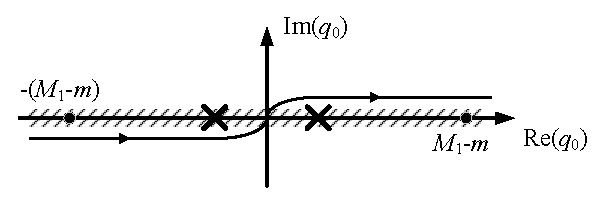
\includegraphics[scale=1.5]{PathIntegrateMode1.eps}
		\caption{Контур интегрирования по $q_0$ в~(\ref{eq:FullIntegrate}) для моды 1. Штрихами показана область нестабильности фотона. Крестиком обозначен полюс, соответствующий $q_0=\omega$ -- вещественному собственному значению поляризационного оператора, точками обозначены полюса.} \label{fig:FullPathIntegrMode1}
	\end{figure}
\end{center}

Аналогично магнитному полю разложим функцию Грина по собственным векторам $r_\alpha^{(\lambda)}$ поляризационного оператора в замагниченной плазме (см. приложение~\ref{app3}):
\begin{equation}\label{eq:InvGcFourier}
	G^C_{\alpha\beta}(x)=\int \frac{\dd^4q}{(2\pi)^4}G^C_{\alpha \beta}(q) e^{-\ii qx}\, ,
\end{equation}
\begin{equation}\label{eq:GcFourier}
	G^C_{\alpha\beta}(q)=\sum_{\lambda=1}^{3}\frac{r_\alpha^{(\lambda)}r^{(\lambda)}_\beta}{(r^{(\lambda)})^2}\cdot \frac{1}{q^2-{\cal P}^{(\lambda)}(q)}\, ,
\end{equation}
где ${\cal P}^{(\lambda)}(q)$ -- собственные значения поляризационного оператора в замагниченной плазме.

Далее, подставляя выражение~(\ref{eq:RetSol}) в (\ref{eq:WaveEq}) с учетом~(\ref{eq:RetCasualGreen})--(\ref{eq:GcFourier}), получим следующий результат:
\begin{equation}\label{eq:ASolvePlasma}
	{\cal A}_\alpha(x) = 2 e^{i \mathbf{kx}} \mathrm{Re} \sum_{\lambda=1}^3 \int\frac{\dd q_0}{2\pi i}\frac{r_\alpha^{(\lambda)}(r^{(\lambda)} j)}{(r^{(\lambda)})^2}\frac{e^{-i q_0 t}}{(q_0-i\varepsilon)(q_0^2-\mathbf{k}^2-{\cal P}^{(\lambda)}(q))}\, .
\end{equation}

Как было отмечено в главе 1 и показано в приложении~\ref{app3}, в случае сильно замагниченной плазмы $\beta\gg T^2$ и $\mu=0$ собственные вектора поляризационного оператора фотона приближенно будут такими же, как и в чистом магнитном поле, поэтому перепишем~(\ref{eq:ASolve}) в виде:

\begin{equation}\label{eq:ASolve}
	{\cal A}_\alpha(x) = 2 e^{i \mathbf{kx}} \mathrm{Re} \sum_{\lambda=1}^3 \int\frac{\dd q_0}{2\pi i}\frac{\varepsilon_\alpha^{(\lambda)}(\varepsilon^{(\lambda)} j)}{(\varepsilon^{(\lambda)})^2}\frac{e^{-i q_0 t}}{(q_0-i\varepsilon)(q_0^2-\mathbf{k}^2-{\cal P}^{(\lambda)}(q))}\, .
\end{equation}

В силу линейного характера уравнения~(\ref{eq:WaveEq}), решение~(\ref{eq:ASolve}) для двух возможных поляризаций можно представить в виде:
\begin{equation}\label{eq:ASoveDivide}
	{\cal A}_\alpha(x)={\cal A}^{(1)}_\alpha(x)+{\cal A}^{(2)}_\alpha(x)\, ,
\end{equation}
где 
%
\begin{eqnarray}                        		
{\cal A}^{(\lambda)}_{\alpha} (x) = V^{(\lambda)}_\alpha (0, {\bf x}) \, \text{Re} F^{(\lambda)} (t) \, ,
\label{eq:V}
\end{eqnarray}
\begin{eqnarray}
V^{(\lambda)}_\alpha (0, {\bf x}) = 2\, e^{ i\, {\bf k x}} \, 
\varepsilon^{(\lambda)}_\alpha \, (\varepsilon^{(\lambda)} j)\, .
\label{eq:partialV}
\end{eqnarray}
%
%\beq
%V^{(2)}_\alpha (0, {\bf x}) = 2\, e^{ i\, {\bf k x}} \, \varepsilon^{(2)}_\alpha \, \frac{(q \tilde \varphi j)}{\sqrt{q^2_{\mprl}}} \, .
%\label{eq:partialV2}
%\eeq
%Для дальнейшего анализа, контур интегрирования удобно
%преобразовать в контур, изображенный на рис.11. 

Как следует из~(\ref{eq:ASoveDivide}) и~(\ref{eq:ASolve}) характер распространения фотона в сильно замагниченной плазме будет полностью определяться функцией $F^{(\lambda)} (t)$, которую удобно представить в виде Фурье-интеграла

\begin{equation}\label{eq:FullIntegrate}
	F^{(\lambda)}(t)=\int_C\frac{dq_0}{2\pi \ii}\frac{e^{-\ii q_0 t}}{(q_0-\ii \varepsilon)(q_0^2-\vec{k}^2-{\cal P}^{(\lambda)}(q))}.
\end{equation}

	\begin{figure}[t]\centering
		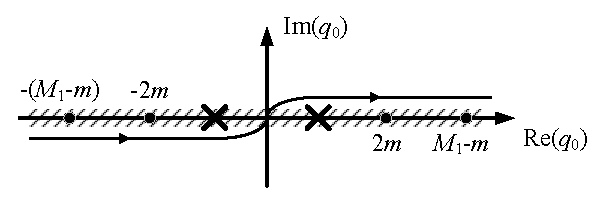
\includegraphics[scale=1.5]{PathIntegrateMode2.eps}
		\caption{Контур интегрирования по $q_0$ в~(\ref{eq:FullIntegrate}) для моды 2. Штрихами показана область нестабильности фотона. Крестиком обозначен полюс, соответствующий $q_0=\omega$ -- вещественному собственному значению поляризационного оператора.}\label{fig:FullPathIntegr}.
	\end{figure}

Контур интегрирования $C$ определяется согласно аналитическим свойствам подынтегрального выражения. В частности, в точке $q_0=\omega$ подынтегральное выражение~(\ref{eq:FullIntegrate}) имеет полюс, который соответствует уравнению дисперсии:

\begin{equation}
	\omega^2 - \vec{k}^2 - {\cal P^{(\lambda)}}(q)=0.
\end{equation}

С другой стороны, как было показано в работе~\cite{MikhChist:2001}, собственные значения поляризационного оператора как в магнитном поле, так и в замагниченной плазме помимо полюсов $q_{\mprl}^2=(M_n\pm M_\ell)^2$, отмеченных в главе 1 настоящей диссертации, также имеют разрезы, которые связаны с распадом фотона на $e^+e^-$-пару и переходом электрона на другие уровни Ландау, т. е. соответствуют областям нестабильности фотона (см. рис.~\ref{fig:FullPathIntegrMode1} и~\ref{fig:FullPathIntegr}). С учетом этих особенностей  контур интегрирования может быть определен, как показано на~рис.~\ref{fig:FullPathIntegrMode1}~и~\ref{fig:FullPathIntegr}.

Следует отметить, что в сильно замагниченной плазме в кинематической области $q_0<2m$ мнимая часть поляризационного оператора для обеих мод пренебрежимо мала по сравнению с реальной частью (влияние резонансов отсутствует), поэтому для удобства контур интегрирования как для фотона моды~1, так и для фотона моды 2 можно преобразовать согласно рис.~\ref{fig:PathIntegr}. Таким образом, интеграл~(\ref{eq:FullIntegrate}) можно представить в виде двух слагаемых
\begin{eqnarray}
F^{(\lambda)}(t) = F^{(\lambda)}_{pole}(t) + F^{(\lambda)}_{cut}(t),
\label{eq:19}
\end{eqnarray}
%
первое из которых определяется вычетом в точке $q_0 = \omega$, являющейся
решением уравнения дисперсии $q^2 - {\cal P}^{(\lambda)}(q) = 0$ в кинематической области, где собственное 
значение поляризационного оператора фотона ${\cal P}^{(\lambda)}(q)$ -- вещественно. 

%Оно соответствует незатухающему
%решению в области $\omega < 2 m$~\cite{Shab}.
Второе слагаемое определяет зависимость потенциалов ${\cal A}^{(\lambda)}_\alpha(x)$ от времени
в области $q_0>2m$ и имеет вид
фурье-интеграла:
%
\begin{eqnarray}
F^{(\lambda)}_{cut}(t) &=& \int \limits_{- \infty}^{\infty} \frac{dq_0}{2 \pi}\,
F^{(\lambda)}_{cut}(q_0)e^{- i q_0 t},
\label{eq:20} 
\\
F^{(\lambda)}_{cut}(q_0) &\simeq& 
\frac{2 \,\theta (q_0  -  2 m)\,I^{(\lambda)}}
{q_0\,([ q_0^2 - {\bf k}^2 - R^{(\lambda)}]^2 + [I^{(\lambda)}]^2)},
\label{eq:21}
\end{eqnarray}
%
где $R \equiv \text{Re} {\cal P}^{(\lambda)}(q_0)$  – реальная, $I \equiv  - \text{Im} {\cal P}^{(\lambda)}(q_0 + i \varepsilon)$ – мнимая 
части поляризационного оператора фотона в замагниченной плазме.
\newpage
Мнимая часть поляризационного оператора может быть получена из коэффициента  
поглощения фотона и представлена в следующем виде:
\begin{eqnarray}
W^{(\lambda)}_{abs} = W_{\gamma^{(\lambda)} \to e^+ e^-} + W_{\gamma^{(\lambda)} e^{\pm} \to e^{\pm}} \, .
\label{eq:Wabs}
\end{eqnarray}
где $W_{\gamma^{(\lambda)} \to e^+ e^-}$ -- коэффициент поглощения фотона в процессе однофотонного рождения электрон-позитронной пары, $W_{\gamma^{(\lambda)} e^{\pm} \to e^{\pm}}$ -- коэффициент поглощения фотона в процессе поглощения фотона электроном.

\begin{figure}[t]\centering
	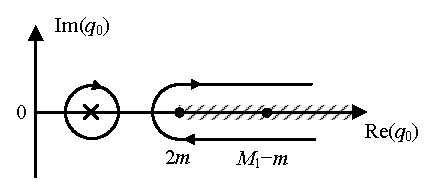
\includegraphics[scale=1.5]{PathIntegrate2Gl.eps}
	\caption{Контур интегрирования по $q_0$ в~(\ref{eq:20}) для мод $\lambda = 1,2$. Штриховой линией показана область, где мнимая часть поляризационного оператора двух возможных мод $\lambda = 1,2$ существенна. Остальные обозначения аналогичны~рис.~\ref{fig:FullPathIntegr}.}\label{fig:PathIntegr}
\end{figure}

С учетом процессов излучения фотонов, (\ref{eq:Wabs}) может быть представлена в следующей форме (см., например,~\cite{Shabad:1988, Rumyantsev:2017,Weldon:1983}): 
\begin{eqnarray}\label{eq:Ilambda}
I^{(\lambda)}=\text{Im} {\cal P}^{(\lambda)} =  -2 q_0 [1-\exp (-q_0/T)] W^{(\lambda)}_{abs} \, . 
\label{eq:ImP}
\end{eqnarray}

Значения $W_{\gamma^{(1)} \to e^+ e^-}$ могут быть получены из~(\ref{eq:wabs1})
с использованием перекрестной симметрии:
\begin{equation}\label{eq:Wgamma1epem}
	\begin{gathered}
		W_{\gamma^{(1)}\to e^+e^-}= \frac{\alpha\beta }{q_0}\sum_{\ell, \ell'=0}^{\infty}\frac{[1-f_{E_{\ell}}][1-f_{q_0-E_\ell}]}{\sqrt{\left( M_{\ell'}^2-M_\ell^2-q_0^2\right)^2-4q_0^2 M_\ell^2}}\times
		\\
		\times \left\{\left(2\beta  ({\ell'}+\ell)-q_0^2\right)\left({\cal I}_{{\ell'},\ell-1}^2+{\cal I}_{{\ell'}-1,\ell}^2\right)-
		8 \beta  \sqrt{l n} {\cal I}_{{\ell'},\ell} {\cal I}_{{\ell'}-1,\ell-1}
		\right\}\, ,
	\end{gathered}
\end{equation}
где ${\cal I}_{n, \ell}\equiv{\cal I}_{n, \ell}(\frac{q_\perp^2}{2\beta})$.

\newpage
Из~(\ref{eq:Wgamma1epem}) следует, что для фотона моды 1 коэффициент поглощения для процесса рождения электрон-позитронной пары на уровнях Ландау $\ell=\ell'=0$ равен нулю. Для фотона моды 2 из~(\ref{eq:wabs2}) получим:
\begin{equation}
\begin{gathered}
%W_{\gamma^{(2)}\to e^+e^-}=\frac{\alpha\beta}{2}\frac{1}{M_{\ell'}q_0^2}\frac{1}{q_0\sqrt{(q_0^2-(M_\ell^2+M_{\ell'}^2))^2-4M_\ell^2M_{\ell'}^2}}\frac{1}{q_0^2-(M_\ell+M_{\ell'})^2}\times
%\\
%\times\bigg(
%(q_0^2+(M_\ell^2-M_{\ell'}^2))^2 M_{\ell'}(M_\ell^2+M_{\ell'}^2+2m^2)
%-
%2M_\ell (M_\ell+M_{\ell'})^2(m^2+3M_\ell M_{\ell'})q_0^2\bigg)\times
%\\
%\times[{\cal I}_{\ell,\ell'}^2+{\cal I}_{\ell-1,\ell'-1}^2] - 4M_{\ell'} q_0^2 (q_0^2-(M_\ell+M_{\ell'})^2)2\beta \sqrt{\ell \ell'} {\cal I}_{\ell\ell'} I_{\ell-1,\ell'-1}\\
W_{\gamma^{(2)}\to e^+e^-}= \frac{\alpha\beta }{q_0}\sum_{\ell, \ell'=0}^{\infty}\frac{[1-f_{E_\ell}][1-f_{q_0-E_\ell}]}{\sqrt{\left( M_{\ell'}^2-M_\ell^2-q_0^2\right)^2-4q_0^2 M_\ell^2}}\times
\\
\times \left\{\left(\frac{\left[2\beta  ({\ell'}-{\ell'})\right]^2}{q_0^2}-2 \beta  (\ell+{\ell'})-4m^2\right)\left({\cal I}_{{\ell'},\ell}^2+{\cal I}_{{\ell'}-1,\ell-1}^2\right)-
8 \beta  \sqrt{\ell {\ell'}} {\cal I}_{{\ell'},\ell} {\cal I}_{{\ell'}-1,\ell-1}
\right\}\, .
\end{gathered}
\end{equation}


Реальная часть 
поляризационного оператора может быть восстановлена по его мнимой части с помощью дисперсионного соотношения с одним 
вычитанием:
%
\beq 
R^{(\lambda)}=\textrm{Re}{\cal P}^{(\lambda)} (t) = \int \limits_0^\infty \frac{\textrm{Im}({\cal P}^{(\lambda)} (t'))\,dt'}{t'-t-i o} - \textrm{Re}{\cal P}^{(\lambda)} (0)\,, \qquad  t = q^2_0 \, .
\label{eq:Disp}
\eeq

В общем случае произвольных уровней Ландау $\ell$ и $\ell'$ задача о вычислении $\textrm{Re} {\cal P}^{(\lambda)}(t)$ выглядит очень громоздко, поэтому в сильно замагниченной плазме можно ограничиться вкладом только первых двух уровней Ландау, которые для области $q_0>2m$ будут выглядеть следующим образом:
\beq
&&W_{\gamma^{(1)} e \to e} \simeq \frac{\alpha \beta}{q_0}
%\times 
%\\
%\nonumber
%&&\times 
\frac{f_{E_{0}} (1 - f_{E_{0} + q_0})}{\sqrt{(2\beta-q^{2}_{0})^2-4 q^{2}_{0}m^2}} (2 \beta - q^{2}_{0}) e^{-\frac{q_0^2}{2\beta}}   \, ,
\eeq
%

\beq
\label{eq:wabs2} 
&&W_{\gamma^{(2)} e \to e} \simeq
\frac{\alpha \beta}{q_0} 
%\times 
%\\
%\nonumber
%&&\times 
\frac{f_{E_{0}} (1 - f_{E_{1} + q_0})}{\sqrt{(2\beta-q^{2}_{0})^2-4 q^{2}_{0}m^2}}
\left (\frac{4\beta^2}{q^{2}_{0}} - 2 \beta - 4 m^2 \right )
\frac{q_0^2}{2\beta} e^{\frac{q_0^2}{2\beta}}\, ,
\eeq
\begin{equation}\label{eq:Wgam2ee}
	\begin{aligned}
			&W_{\gamma^{(2)} \to e^+e^-} \simeq\frac{\alpha \beta}{q_0}e^{\frac{q_0^2}{2\beta}} \bigg\{
		\frac{(1-f_{E_{0}}) (1 - f_{q_0 - E_{0}})}{q_0\sqrt{q^{2}_{0}-4 m^2}}
		\left (- 4 m^2 \right )+
		\\
		& 
		+
		\frac{q_0^2}{\beta}
		%\times 
		%\\
		%\nonumber
		%&&\times 
		\frac{(1-f_{E_{0}}) (1 - f_{q_0 - E_{1}})}{\sqrt{(2\beta-q^{2}_{0})^2-4 q^{2}_{0}m^2}} 
		\left (\frac{4\beta^2}{q^{2}_{0}} - 2 \beta - 4 m^2 \right ) 
		%\times 
		%\\
		%\nonumber
		%&& \times 
		 \bigg\} \, ,
	\end{aligned}
\end{equation}
где
\beq
\nonumber
&&E_{n} = \frac{1}{2 q_{0}} \,\left|2\beta n - q^2_{0}\right |\, .
\eeq

В результате выражения для мнимой и действительной частей поляризационного оператора для фотонов моды 1 и моды 2 с учетом~(\ref{eq:Ilambda}--\ref{eq:Wgam2ee}) и магнитного поля при условии $q_0^2>4m^2$ удобно представить следующим образом:

\begin{equation}
I^{(1)}=2\alpha\beta\exp \left[-\frac{q_\perp^2}{2\beta }\right]\frac{\left(2\beta -q_0^2\right) f_{E_0}\left(1-f_{E_0+q_0}\right)\left(1-\exp[q_0/T]\right)}{ \sqrt{\left((M_1-m)^2-q_0^2\right) \left((M_1+m)^2-q_0^2\right)}}
\end{equation}

\begin{equation}\begin{aligned}
R^{(1)}&= -\frac{\alpha \beta}{2\pi}\exp\left[\frac{-q_\perp^2}{2\beta}\right]\bigg(\frac{M_1^2-m^2-q_0^2}{\sqrt{((M_1+m)^2-q_0^2)((M_1-m)^2-q_0^2)}}
\times
\\
&\times
\ln\left[\frac{\sqrt{(M_1+m)^2-q_0^2}+\sqrt{(M_1-m)^2-q_0^2}}{2\sqrt{M_1 m}}\right]-\ln\left[\frac{M_1^2}{m^2}\right]\bigg)
-
\\
&-\frac{\alpha \beta q_0^2 m^2}{2\pi} \exp\left[-\frac{q_\perp^2}{2\beta}\right]\int_{0}^{\infty}\frac{\dd z}{\exp \left[\frac{m}{T}\sqrt{z^2+1}\,\right]+1}\times
\\
&\times\frac{\sqrt{z^2+1}}{ \left(M_1^2-m^2-q_0^2\right)^2-4m^2q_0^2 \left(z^2+1\right)}\, ,
\end{aligned}
\end{equation}

\begin{equation}\begin{aligned}
I^{(2)}=&-2\alpha\beta\left(1-\exp\left[{\frac{-q_0}{T}}\right]\right)\exp\left[{\frac{-q^2_\perp}{2\beta}}\right] \bigg\{
\frac{(1-f_{E_{0}}) (1 - f_{q_0 - E_{0}})}{q_0\sqrt{q^{2}_{0}-4 m^2}}
\left (- 4 m^2 \right )+
\\
& 
+
\frac{q_0^2}{\beta}
%\times 
%\\
%\nonumber
%&&\times 
\frac{4\beta^2/q^{2}_{0} - 2 \beta - 4 m^2}{\sqrt{((M_1+m)^2-q_0^2)((M_1-m)^2-q_0^2)}}\times
\\
&\times\bigg[(1-f_{E_{0}}) (1 - f_{q_0 - E_{1}})+
\frac{1}{2}f_{E_{0}} (1 - f_{E_{1} + q_0})
\bigg]
\bigg\}\, ,
\end{aligned}\end{equation}

\begin{equation}\begin{aligned}
	R^{(2)}&= \frac{\alpha\beta}{2\pi}\exp\left[-\frac{q_\perp^2}{2\beta}\right]\left(\frac{4m^2}{\sqrt{q_0^2(q_0^2-4m^2)}}\ln\left[\frac{\sqrt{q_0^2}+\sqrt{q_0^2-4m^2}}{4m^2}\right]+1\right)+ 
	\\
	&+\frac{\alpha}{16\pi}q^2_\perp \exp\left[-\frac{q_\perp^2}{2\beta}\right] \bigg( \frac{4m^2+2\beta+\frac{4\beta^2}{ q_0^2}}{\sqrt{((M_1-m)^2-q^2_0)((M_1-m)^2-q^2_0)}}
	\times
	\\
	&\times
	\ln\left[\frac{\sqrt{(M_1+m)^2-q_0^2}+\sqrt{(M_1-m)^2-q_0^2}}{2(m^4+2\beta m^2)^{1/4}}\right]+
	\\
	&+\frac{1}{2}\left(\frac{m^2}{\beta}-\frac{2\beta}{q_0^2}\right)\ln\left[\frac{m^2+2\beta}{m^2}\right]+1\bigg)- \frac{4\alpha\beta m^2}{\pi}\exp\left[-\frac{q_\perp^2}{2\beta}\right]\times
	\\
	&\times
	\int_{0}^{\infty}\frac{1}{\sqrt{1+z^2}}\frac{1}{\exp[\frac{m}{T}\sqrt{(1+z^2)}\,]+1}\bigg(\frac{1}{q_0^2-4m^2(1+z^2)}+
	\\
	&+\frac{q_0^2}{\beta}\frac{2\beta z^2 + q_0^2}{(2\beta - q_0^2)^2-m^2(1+z^2)q_0^2}\bigg)\dd z\, .
\end{aligned}\end{equation}

Следует отметить, что в поставленной задаче рассматриваются процессы только до второго циклотронного резонанса $q_0=M_1-m$, поэтому те же процессы с другими уровнями Ландау вклада не дают.

Выражения (\ref{eq:20})-(\ref{eq:Wabs}) с учетом (\ref{eq:Disp}) решают задачу 
о нахождении временной зависимости волновой функции фотона  в присутствии сильно 
замагниченной плазмы. 

\begin{figure}[t!]\centering
	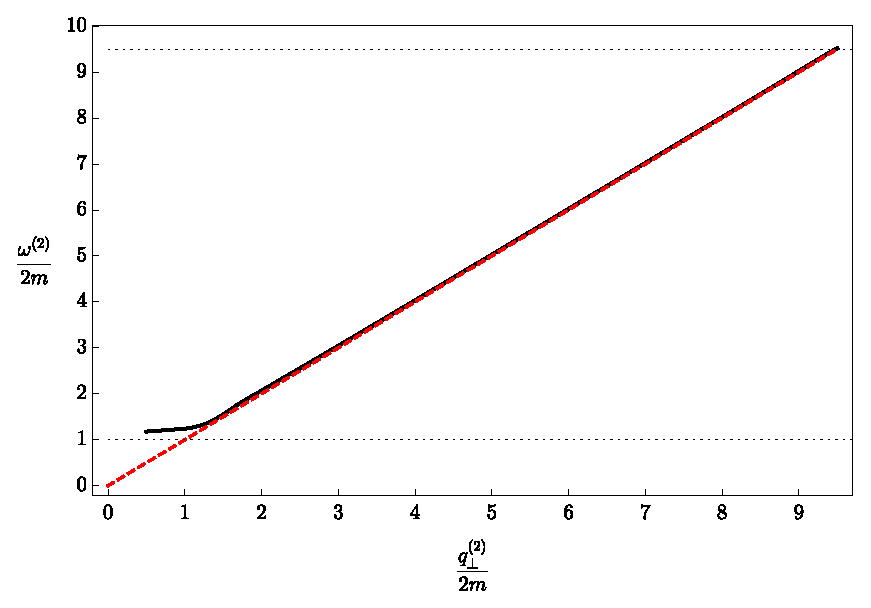
\includegraphics[scale=1.2]{DisperseMode2.eps}
	\caption{Дисперсия фотона моды 2 в области нестабильности, связанной с процессами распада на $e^+e^-$ пару и поглощения $e_0 \gamma^{(2)}\to e_1$, представлена сплошной линией при магнитном поле $B=200B_e$ и $T=1$~МэВ. Штриховая линия соответствует вакуумному закону дисперсии. Пунктирные линии обозначают пороги $\omega^{(2)}=2m$ и $\omega^{(2)}=M_1-m$. \label{fig:DisperseMode2}}
\end{figure}

Временную часть волновой функции фотона $F(t)$ можно представить в виде затухающих колебаний для мод $\lambda=1,2$:
\begin{equation}\label{eq:Fm}
	F^{(\lambda)}(t)\sim F^{(\lambda)}_A(t) \cos(\omega^{(\lambda)} t+\phi_0)
\end{equation}
где $F^{(\lambda)}_A(t)$ -- амплитуда колебаний,
временная зависимость которой определяет
характер затухания волновой функции,
$\omega^{(\lambda)}$ -- эффективная
частота. В работе~\cite{Shabad:1988}
предполагался экспоненциальный характер затухания с декрементом затухания, равным мнимой части энергии фотона, полученным из решения уравнения дисперсии на втором римановом листе. Анализ  аналитических свойств фурье-образа $F^{(\lambda)}_{cut}(q_0)$ показывает, что характер временного затухания волновой функции в общем случае является неэкспоненциальным. Тем не менее на протяжении некоторого характерного отрезка времени $(\sim [W^{(\lambda)}_{abs}]^{-1})$
зависимость волновой функции от времени можно приближенно описать как 
экспоненциально затухающие гармонические колебания:
%
\begin{equation}\label{eq:ApproxA}
{\cal A}^{(\lambda)}_\mu(t) \sim e^{- \gamma^{(\lambda)}_\text{eff} \, t/2} \cos 
(\omega^{(\lambda)} t + \phi_0).
\end{equation}
%
Здесь $\omega^{(\lambda)}$ и $\gamma^{(\lambda)}_\text{eff}$ -- эффективная 
частота и коэффициент  
поглощения фотона моды $\lambda$ соответственно, которые должны быть найдены с использованием 
(\ref{eq:20})--(\ref{eq:Wabs}) для каждого значения импульса ${\bf k}$, что определяет эффективный 
закон дисперсии фотона в области его нестабильности~(см. рис.~\ref{fig:DisperseMode1} и \ref{fig:DisperseMode2}).


\subsection{Численный анализ}



\begin{figure}[t]\centering
	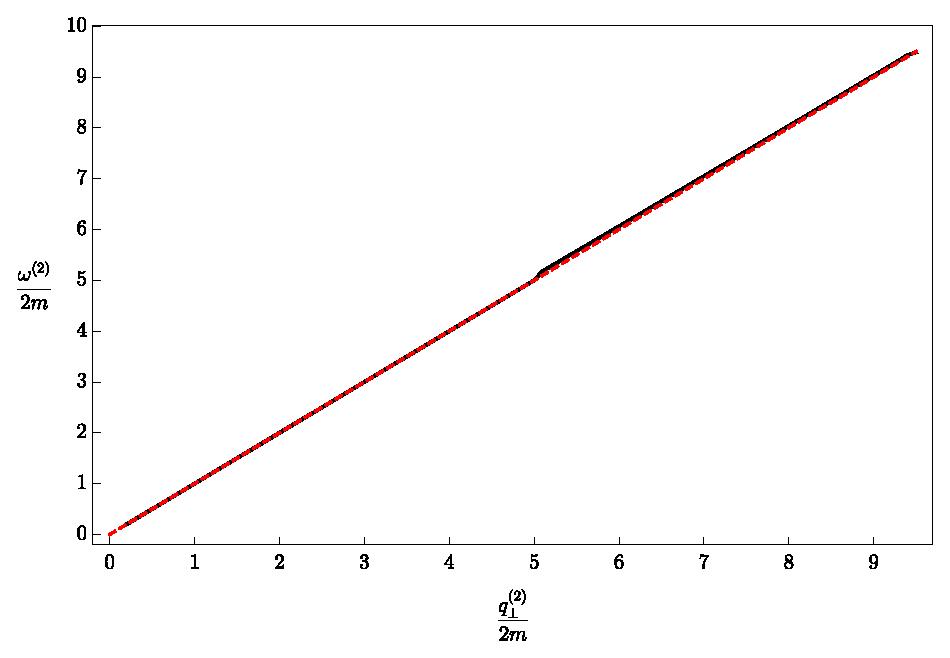
\includegraphics[scale=1.2]{DisperseMode1.eps}
	\caption{Дисперсия фотона моды 1 в области нестабильности, связанной с процессом поглощения $e_0 \gamma^{(1)}\to e_1$ представлена при магнитном поле $B=200B_e$ и $T=1$~МэВ. Пунктирная линия обозначает порог $\omega^{(1)}=M_1-m$ \label{fig:DisperseMode1}}
\end{figure}

Рис.~\ref{fig:DisperseMode1} и ~\ref{fig:DisperseMode2} демонстрируют законы дисперсии фотонов моды 1 и моды~2 в сильно замагниченной плазме при температуре $T = 1$ МэВ и магнитном поле $B = 200B_e$ в области их нестабильности. Из представленных результатов следует, что закон дисперсии для фотона моды 1 в области нестабильности незначительно отличается от вакуумного закона дисперсии~(см.~рис.~\ref{fig:DisperseMode1}). С другой стороны, дисперсионная кривая фотона моды 2 значительно отличается от вакуумной вблизи порога $\omega^{(2)}=4m$ и в малой окрестности порога~$\omega^{(2)}=M_1-m$. Для построения дисперсионной кривой до следующего резонанса необходимо учитывать следующие уровни Ландау. При этом полученная картина дисперсионных кривых согласуется с анализом уравнения дисперсии, выполненного в работе~\cite{Shabad:1988}.


\begin{figure}[t]\centering
	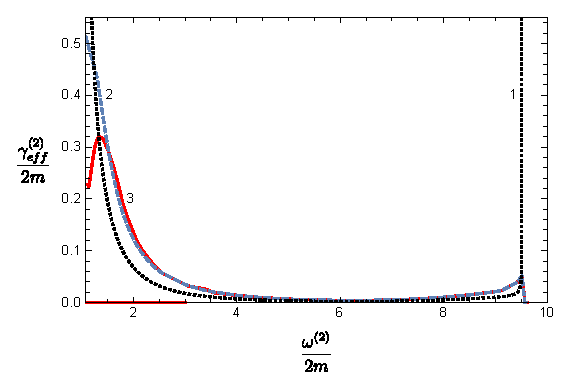
\includegraphics[scale=0.8]{mode2.eps}
	\caption{\label{fig:fig2}Зависимость ширины распада фотона моды 2 от частоты в припороговых областях при $B=200 B_e$, $T=1$ МэВ и $ \mu=0 $. Линия $ {\it 1} $ - коэффициент поглощения фотона $ W ^ {(1)}_{abs} $,
		% в процессах $ \ gamma \ to e ^ + e ^ - $ и $ \ gamma e ^ { \ pm} \ to e ^ {\ pm} $,
		вычисленный в древесном приближении и содержащий корневые особенности; линия $ {\it 2} $ - ширина распада, полученная из комплексного решения дисперсионного уравнения на втором римановом листе [6]; линия $ {\it 3} $ соответствует ширине затухания $ \gamma^{(1)}$, вычисленной на основе приближения~(\ref{eq:ApproxA}).}\label{fig:DampMode2}
\end{figure}

Для астрофизических приложений полезно вычислить величину $\gamma_\text{eff}$, которая определяет интенсивность поглощения 
$\gamma$-квантов в замагниченной плазме за счет  процессов $\gamma \to e^+ e^-$  и $\gamma e^{\pm} \to e^{\pm}$.
Обычно в астрофизике  используют выражение для коэффициента поглощения,
полученное на основе  вероятности распада  $ \gamma \to e^+ e^-$. Однако в околопороговой области эти выражения
содержат корневые сингулярности (см. например~\cite{HBG:1997}), которые были отмечены во введении к данной главе. 

\newpage
Наш анализ показывает, (см. рис.~\ref{fig:DampMode1} и~\ref{fig:DampMode2}),
что вычисление коэффициента  поглощения с учетом неэкспоненциального характера 
затухания приводит к конечному выражению для коэффициента  поглощения фотона в окрестности резонансов 
$q_0 = (\sqrt{m^2+2 \beta} - m )$ как для фотона моды 2, так и для фотона моды 1. Исходя из рис. \ref{fig:DampMode1} можно сделать вывод, что фотон моды 1 является квазистабильным в областях $q_0<7$ МэВ и $q_0>(\sqrt{m^2+2 \beta} - m)\simeq 9.5$~МэВ. С другой стороны, фотон неустойчив в области, близкой в окрестности резонансов $q_0 = (\sqrt{m^2+2 \beta} - m )$. Фотон моды 2 можно считать квазиустойчивым в области $q_0<4m$ и $q_0>(\sqrt{m^2+2 \beta} - m)$. Коэффициент затухания фотона, полученный из результатов работы~\cite{Shabad:1988}, является завышенным в околопороговой области по сравнению с результатами, полученными с помощью аппроксимации~(\ref{eq:ApproxA}). Однако существует область энергий фотона ($2.5\lesssim q_0\lesssim 8.5$ МэВ для фотона моды 2 и $q_0\lesssim8.7$ МэВ для фотона моды 1), где коэффициенты поглощения, полученные из результатов работы~\cite{Shabad:1988} и с помощью аппроксимации~(\ref{eq:ApproxA}) совпадают.


\begin{figure}[t]\centering
	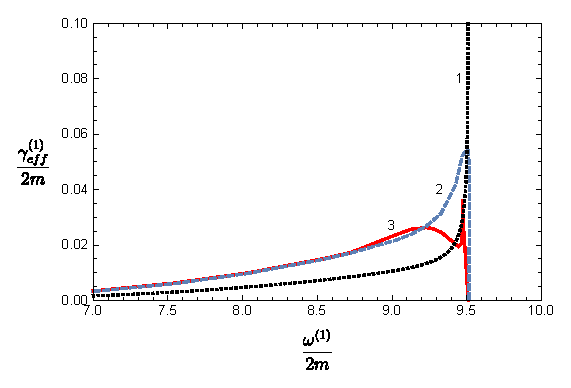
\includegraphics[scale=0.8]{mode1.eps}
	\caption{\label{fig:fig1}Зависимость ширины распада фотона моды 1 от частоты в припороговых областях при $B=200 B_e$, $T=1$ МэВ и $ \mu=0 $. Линия $ {\it 1} $ - коэффициент поглощения фотона $ W ^ {(1)}_{abs} $,
		% в процессах $ \ gamma \ to e ^ + e ^ - $ и $ \ gamma e ^ { \ pm} \ to e ^ {\ pm} $,
		вычисленный в древесном приближении и содержащий корневые особенности; линия $ {\it 2} $ - ширина распада, полученная из комплексного решения дисперсионного уравнения на втором римановом листе [6]; линия $ {\it 3} $ соответствует ширине затухания $ \gamma^{(1)}$, вычисленной на основе приближения~(\ref{eq:ApproxA}).}\label{fig:DampMode1}
\end{figure}

\begin{figure}[t!]\centering
	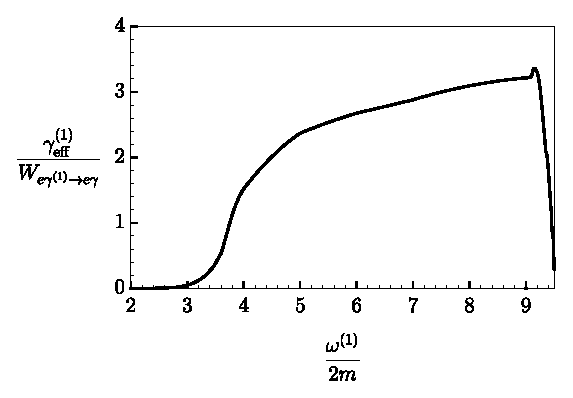
\includegraphics[scale=1.3]{CompareDampAndCompton.eps}
	\caption{\label{fig:ComptonandDamp} Отношение коэффициента затухания фотона $\gamma_{eff}^{(1)}$ к коэффициенту поглощения фотона в процессе $e\gamma^{(1)}\to e\gamma$ при $B=200B_e$ и $T=1$ МэВ}
\end{figure}
\begin{figure}[t!]\centering
	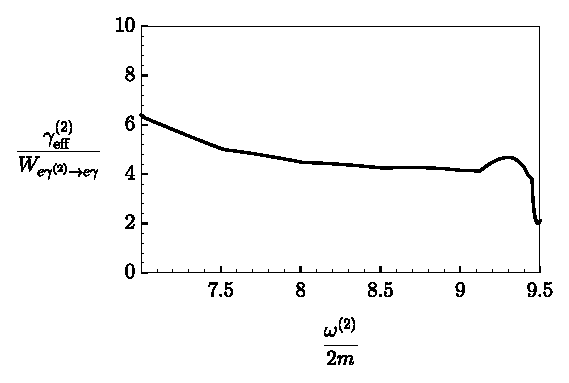
\includegraphics[scale=1.3]{CompareDampAndCompton2.eps}
	\caption{\label{fig:ComptonandDamp2} Отношение коэффициента затухания фотона $\gamma_\text{eff}^{(2)}$ к коэффициенту поглощения фотона в процессе $e\gamma^{(2)}\to e\gamma$ при $B=200B_e$ и $T=1$ МэВ}
\end{figure}
\clearpage

На основе полученных результатов представляет интерес рассмотреть задачу о возможности формировании комптоновского процесса при условии затухания фотона. Для этого удобно вычислить отношение коэффициента затухания фотона к коэффициенту поглощения фотона $e\gamma^{(1)}\to e\gamma$  (см. рис. \ref{fig:ComptonandDamp}), полученном в главе 2 и который определяет время его формирования. Как видно из рисунка~\ref{fig:ComptonandDamp}, комптоновский процесс, несмотря на малый фактор $\alpha$, успевает формироваться при энергиях фотона $\omega\lesssim3$ МэВ. Для фотона моды 2 комптоновский процесс формируется только в области энергий фотона $\omega\lesssim1$ МэВ. В области энергий $\omega>3$ МэВ для моды 1 и $\omega>1$ МэВ фотоны будут эффективно затухать, и комптоновский процесс, по-видимому, не успевает сформироваться. Для моды 2 (см. рис.~\ref{fig:ComptonandDamp2}) даже с учетом области квазистабильности (вдали от порогов), комптоновский процесс будет формироваться только при энергиях фотона~$\omega<1$~МэВ.

Таким образом, коэффициенты поглощения фотона в комптоновском процессе для двух возможных каналов рассеяния $e\gamma^{(1)}  \to e\gamma^{(1)}$ и $e\gamma^{(1)}  \to e\gamma^{(2)}$, несмотря на резонансный характер, целесообразно рассматривать лишь вдали от циклотронных резонансах, поэтому для анализа комптоновского процесса при высоких температурах $T\simeq 1$ МэВ и магнитных полях $B=200 B_e$ достаточно использовать разложение по обратным степеням напряженности магнитного поля~\cite{Chistyakov:2009}. Каналы же рассеяния $e\gamma^{(2)}  \to e\gamma^{(1)}$  и $e\gamma^{(2)}  \to e\gamma^{(2)}$ в области резонанса рассматривать нецелесообразно, так как комптоновский процесс не успевает сформироваться для энергий фотона $\omega\gtrsim 2m$.

\newpage

\subsection{Выводы}
Исследован процесс распространения квантованной электромагнитной волны в сильно замагниченной, зарядово-симметричной плазме. С учетом изменения дисперсионных свойств фотона в магнитном поле и плазме было установлено, что, аналогично случаю чистого магнитного поля процесс затухания фотона
в замагниченной плазме имеет неэкспоненциальный характер. 

Для характерного отрезка времени $\sim [W^{{(\lambda)}}_{abs}]^{-1}$ была использована аппроксимация экспоненциально затухающими колебаниями. В этом случае было
показано, что коэффициент поглощения фотона в околопороговой области меньше по сравнению с известными в литературе результатами. Также, следуя данной аппроксимации, были построены дисперсионные кривые, которые и для моды 1, и для моды 2 близки к вакуумным кривым, за исключением околопороговых областей. Полученные результаты согласуются с выводами работы~\cite{Shabad:1988}.

Для определения характера затухания фотона необходимо выполнить более детальный анализ временной зависимости амплитуды $F_A(t)$ колебаний, входящей в уравнение~(\ref{eq:Fm}). Кроме того, был выполнен анализ возможности формирования комптоновского процесса в условиях нестабильности фотона за счет процесса поглощения электроном $e^\pm\gamma\to e^\pm$ и распада на электрон-позитронную пару $\gamma\to e^+e^-$. Несмотря на малый фактор $\alpha$, комптоновский процесс преобладает над процессами распада и поглощения в области низких энергий фотона ($\omega<3$ МэВ при $T=1$ МэВ и $B =200B_e$). С другой стороны, даже с учетом резонанса на виртуальном электроне, фотоны как моды 1, так и моды~2 в пределе сильного магнитного поля $B=200 B_e$ и температуре $T=1$ МэВ эффективно затухают в резонансной области.
